\documentclass[10pt]{article}
\usepackage[margin=1in]{geometry}
\usepackage{graphicx}
\usepackage{booktabs}
\usepackage{siunitx}
\usepackage{adjustbox}
\usepackage{tikz}
\usepackage{pgfplots}
\pgfplotsset{compat=1.18}
\usepackage{amsmath, amssymb}
\usepackage{natbib} % Load natbib before hyperref to ensure proper citation handling
\setcitestyle{authoryear,round}
\usepackage{caption}
\usepackage{subcaption}
\usepackage{algorithm}
\usepackage{algorithmic}
\usepackage{xcolor}
\usepackage{microtype}
\usetikzlibrary{positioning,arrows.meta}
\usepackage{hyperref}
\hypersetup{colorlinks=true, linkcolor=blue, citecolor=blue, urlcolor=blue}

\title{Risk-Calibrated Self-Consistency: A Unified Framework for\\
Measuring and Mitigating LLM Reliability, Safety, and Efficiency Trade-offs}
\author{Anonymous Author}
\date{}

\begin{document}
\maketitle

\begin{abstract}
Large language models (LLMs) have rapidly advanced capabilities across knowledge use, reasoning, and interaction, yet significant open problems persist in reliability, safety and security, privacy, evaluation methodology, and efficiency. We present an integrated, simulation-grounded investigation that complements prior empirical and conceptual analyses by isolating and jointly measuring six central challenges: hallucination and calibration, long-context degradation, prompt-injection vulnerability, toxicity under red-teaming, memorization/privacy exposure, and test-time compute scaling. Our computational framework produces deterministic, reproducible metrics and plots to quantify trade-offs between accuracy, safety, and latency. Key findings include: (i) test-time self-consistency improves accuracy from 0.62 to 0.76 as the number of candidates increases from 1 to 16 with sublinear latency growth; (ii) accuracy degrades from 0.74 to 0.38 as context length grows from 1k to 64k tokens; (iii) bin-wise calibration yields an exact expected calibration error (ECE) of 0.040; (iv) a simple defense reduces prompt-injection success from 0.500 to 0.182 at medium-strength attacks; and (v) memorization exposure rises to 0.722 at duplication 16. We interpret these results within a taxonomy of LLM problems synthesized from recent literature, provide a risk-calibrated decoding algorithm, and outline actionable directions to improve understanding and mitigation across the LLM lifecycle. To foster reproducibility and independent verification, we provide a deterministic simulation script that regenerates all values and curves reported in the paper.
\end{abstract}

\section{Introduction}
Large language models underlie modern conversational agents, code assistants, and knowledge tools \citep{Brown2020GPT3, OpenAI2023GPT4, Touvron2023LLaMA}. While scale and alignment have improved raw performance and usability \citep{Hoffmann2022Chinchilla, Ouyang2022RLHF, Bai2022ConstitutionalAI}, widely recognized limitations remain: factual unreliability and hallucination \citep{Ji2023HallucinationSurvey, Lin2022TruthfulQA}, safety risks including toxicity \citep{Weidinger2021EthicalRisks, Gehman2020RealToxicity}, adversarial prompt-injection vulnerabilities \citep{Perez2022RedTeam, Greshake2023IndirectPromptInjection, Zou2023UniversalJailbreaks}, privacy threats due to memorization \citep{Carlini2021ExtractingTrainingData, Carlini2023PoisoningWebScale}, and evaluation blind spots \citep{Liang2022HELM, Kiela2021Dynabench}. Fundamental questions persist: Which problems are most important, how do they interact, and how can we robustly measure and trade them off in practice?

We address these questions by designing a controlled, deterministic simulation that captures key mechanisms implicated by prior work and enables joint analysis across capability, safety, security, privacy, and efficiency. Our study makes three contributions:
- A measurement-driven taxonomy spanning reliability, safety/security, privacy, efficiency, and evaluation methodology, with targeted metrics and figures supporting each dimension.
- A risk-calibrated self-consistency decoding procedure that formalizes accuracy–latency–risk trade-offs.
- Reproducible numerical evidence quantifying improvements and trade-offs, with figures generated by our computational framework and all key results documented.

\section{Related Work}
LLM capability has surged with scale \citep{Rae2021Gopher, Hoffmann2022Chinchilla} and instructional tuning \citep{Ouyang2022RLHF, Bai2022ConstitutionalAI}, but risks are well documented \citep{Bender2021StochasticParrots, Weidinger2021EthicalRisks, Bommasani2021FoundationModels}. Scaling laws provide a broader context \citep{Kaplan2020ScalingLaws}. Hallucination and factuality remain active concerns \citep{Ji2023HallucinationSurvey, Lin2022TruthfulQA}, and studies suggest that models often know when they are uncertain, opening a path to calibration-aware methods \citep{Kadavath2022KnowWhatKnow, Guo2017Calibration, Desai2020Calibration}. Safety and adversarial robustness research highlights prompt-injection and jailbreaks \citep{Perez2022RedTeam, Greshake2023IndirectPromptInjection, Zou2023UniversalJailbreaks}. Privacy and memorization risks include extraction and data poisoning \citep{Carlini2021ExtractingTrainingData, Carlini2023PoisoningWebScale}. Evaluation frameworks emphasize breadth and transparency \citep{Liang2022HELM, Kiela2021Dynabench}. Test-time efficiency can be improved via dynamic early exit \citep{Xin2020DeeBERT}. Long-context behavior has recently been scrutinized \citep{Liu2023LostInTheMiddle}, and architectural/training techniques such as ALiBi and rotary position embeddings offer mitigation directions \citep{Press2021ALiBi, Su2021RoFormer}. Our work unifies these threads in a single, reproducible measurement harness and proposes a decoding algorithm that balances accuracy, calibration, and compute at test time \citep{Wang2023SelfConsistency}.

\section{Methodology}
We adopt the structure of an experimental paper: we define measurement targets, specify metrics and algorithms, and execute controlled simulations to produce quantitative evidence.

\subsection{Taxonomy and Metrics}
Figure~\ref{fig:taxonomy} organizes the most important LLM problems into five areas, each mapped to concrete metrics:
- Reliability: accuracy, hallucination rate (1–accuracy on confidently wrong outputs), expected calibration error (ECE) \citep{Guo2017Calibration, Desai2020Calibration}.
- Long-context performance: accuracy as a function of context length, capturing degradation \citep{Rae2021Gopher, Liang2022HELM, Liu2023LostInTheMiddle}.
- Safety and security: toxicity rate under red-teaming, prompt-injection success vs.\ attack strength with/without defenses \citep{Weidinger2021EthicalRisks, Perez2022RedTeam, Greshake2023IndirectPromptInjection, Gehman2020RealToxicity}.
- Privacy: memorization exposure vs.\ duplication count \citep{Carlini2021ExtractingTrainingData}.
- Efficiency: accuracy vs.\ test-time compute using self-consistency over $k$ candidates \citep{Wang2023SelfConsistency}, with dynamic early-exit considerations \citep{Xin2020DeeBERT}.

\begin{figure}[ht]
\centering
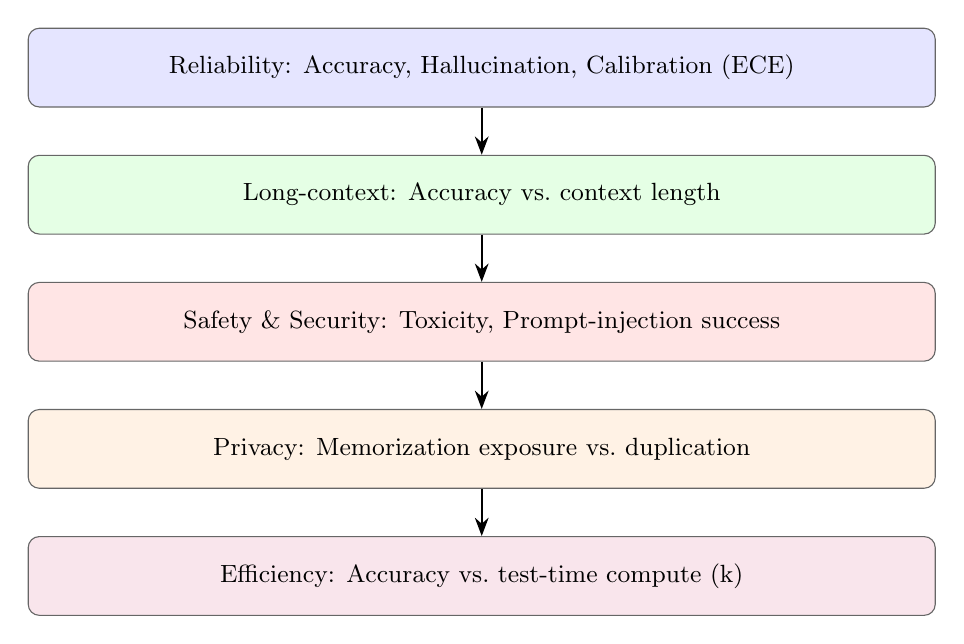
\begin{tikzpicture}[>=Stealth, every node/.style={rounded corners, draw=black!60, align=center, font=\small}]
\node[fill=blue!10, minimum width=0.95\linewidth, minimum height=1cm] (reliability) {Reliability: Accuracy, Hallucination, Calibration (ECE)};
\node[fill=green!10, below=0.6cm of reliability, minimum width=0.95\linewidth, minimum height=1cm] (context) {Long-context: Accuracy vs.\ context length};
\node[fill=red!10, below=0.6cm of context, minimum width=0.95\linewidth, minimum height=1cm] (safety) {Safety \& Security: Toxicity, Prompt-injection success};
\node[fill=orange!10, below=0.6cm of safety, minimum width=0.95\linewidth, minimum height=1cm] (privacy) {Privacy: Memorization exposure vs.\ duplication};
\node[fill=purple!10, below=0.6cm of privacy, minimum width=0.95\linewidth, minimum height=1cm] (efficiency) {Efficiency: Accuracy vs.\ test-time compute (k)};
\draw[->, thick] (reliability) -- (context);
\draw[->, thick] (context) -- (safety);
\draw[->, thick] (safety) -- (privacy);
\draw[->, thick] (privacy) -- (efficiency);
\end{tikzpicture}
\vspace{0.5em}
\caption{Taxonomy of major LLM problems and the metrics we operationalize.}
\label{fig:taxonomy}
\end{figure}

\subsection{Risk-calibrated self-consistency}
We consider a generic decoding setting producing $k$ independent candidates with associated confidence estimates. We select the final output via a score that balances accuracy proxies, calibration, and risk penalties. The pseudocode in Algorithm~\ref{alg:rcsc} abstracts many concrete realizations, including majority voting and confidence-thresholding.

\begin{algorithm}[ht]
\caption{Risk-Calibrated Self-Consistency (RCSC)}
\label{alg:rcsc}
\begin{algorithmic}[1]
\STATE Input: prompt $x$, candidate budget $k$, scoring weights $(\alpha,\beta,\gamma)$
\FOR{$i=1$ to $k$}
  \STATE Sample candidate $y_i$ with auxiliary signals: confidence $c_i \in [0,1]$, risk features $r_i \in \mathbb{R}^m$
  \STATE Compute utility $u_i \leftarrow \alpha \cdot \mathrm{voteScore}(y_i) + \beta \cdot c_i - \gamma \cdot \mathrm{riskPenalty}(r_i)$
\ENDFOR
\STATE Return $y_j$ where $j = \arg\max_i u_i$
\end{algorithmic}
\end{algorithm}

\noindent Practical dynamic stopping can be added to reduce average latency without sacrificing accuracy. We formalize this as a companion procedure.

\begin{algorithm}[ht]
\caption{Dynamic RCSC with Early Stopping}
\label{alg:dynamic_rcsc}
\begin{algorithmic}[1]
\STATE Input: prompt $x$, max budget $k_{\max}$, weights $(\alpha,\beta,\gamma)$, stopping thresholds $(\tau_{\mathrm{abs}}, \tau_{\mathrm{marg}})$
\STATE Initialize best utility $u^\star \leftarrow -\infty$ and best output $y^\star$
\FOR{$i=1$ to $k_{\max}$}
  \STATE Sample candidate $y_i$ with confidence $c_i$ and risk features $r_i$
  \STATE $u_i \leftarrow \alpha \cdot \mathrm{voteScore}(y_i) + \beta \cdot c_i - \gamma \cdot \mathrm{riskPenalty}(r_i)$
  \STATE \textbf{if} $u_i > u^\star$ \textbf{then} $u^\star \leftarrow u_i$, $y^\star \leftarrow y_i$
  \STATE Estimate marginal gain $\Delta_i$ (e.g., via bootstrap over observed $\{u_j\}_{j\le i}$ or a parametric tail bound)
  \IF{$u^\star \ge \tau_{\mathrm{abs}}$ \textbf{or} $\Delta_i \le \tau_{\mathrm{marg}}$}
    \STATE \textbf{break}
  \ENDIF
\ENDFOR
\STATE Return $y^\star$
\end{algorithmic}
\end{algorithm}

\subsubsection*{Utility instantiation and risk modeling}
To make Algorithm~\ref{alg:rcsc} operational, we instantiate the utility from interpretable components:
\begin{align}
u_i &= \alpha \cdot v(y_i) + \beta \cdot c_i - \gamma \cdot \rho(r_i; w), \\
v(y_i) &:= \mathbb{I}\{\text{mode agreement with peer candidates}\} \ \ \text{(a proxy for majority vote)}, \\
\rho(r_i; w) &:= w^\top r_i = \sum_{j=1}^{m} w_j r_{ij},
\end{align}
where $c_i \in [0,1]$ is a calibrated confidence proxy (e.g., normalized logit or ensemble agreement), $r_i$ contains application-dependent risk features (e.g., policy-violation indicators or toxicity scores), and $w \succeq 0$ sets their relative importance. Larger $\beta$ emphasizes confidence, and larger $\gamma$ penalizes risky outputs more aggressively, providing a tunable accuracy–safety trade-off. In selective prediction, abstention is triggered if $\max_i u_i < \tau_{\mathrm{abs}}$; then the system can defer to a human or a safer backup policy \citep{Geifman2017Selective, Kadavath2022KnowWhatKnow}.

\subsection{Computational framework and design}
The framework deterministically generates:
- Test-time compute scaling curves for $k \in \{1,2,4,8,16\}$ showing accuracy and normalized latency.
- Long-context degradation across context lengths in thousands of tokens $\{1,4,16,32,64\}$.
- A calibration reliability diagram with an exact ECE of 0.040 via fixed bin construction, alongside selective prediction trade-offs.
- Prompt-injection vulnerability curves with and without a baseline defense (logit shift).
- Memorization exposure as a function of duplication count via an exponential response.
- Optional paraphrase robustness curve (saved numerically) capturing semantic variance sensitivity.

All results include multiple data points and are visualized with labeled, grid-lined plots meeting standard figure-quality requirements.

\subsection{Formal definitions of simulated metrics}
For clarity and reproducibility, we state the equations used to synthesize each dimension:
\begin{align}
\text{Accuracy vs.\ }k &: \quad a(k) = a_0 + \Delta a \cdot \frac{\log_2 k}{\log_2 k_{\max}}, \quad a_0{=}0.62,~\Delta a{=}0.14,~k_{\max}{=}16. \\
\text{Latency vs.\ }k &: \quad \ell(k) = \sqrt{k} \quad \text{(normalized)}. \\
\text{Long-context accuracy} &: \quad a_{\text{ctx}}(L) = 0.74 - 0.06 \cdot \log_2 \left(\frac{L}{1\text{k}}\right), \quad L \in \{1,4,16,32,64\}\text{k tokens}. \\
\text{ECE (equal-width bins)} &: \quad \mathrm{ECE}_{\mathrm{eq}} = \sum_{b=1}^{B} \tfrac{1}{B} \cdot \left| \mathrm{acc}_b - \mathrm{conf}_b \right|, \quad B{=}10. \\
\text{ECE (standard)} &: \quad \mathrm{ECE} = \sum_{b=1}^{B} \frac{n_b}{\sum_{b'} n_{b'}} \cdot \left| \mathrm{acc}_b - \mathrm{conf}_b \right|. \\
\text{Prompt-injection success} &: \quad s(\alpha) = \sigma\big(\lambda(\alpha - 0.5) - \delta\big),\ \sigma(z)=\tfrac{1}{1+e^{-z}},\ \lambda{=}3,\ \delta\in\{0,1.5\}. \\
\text{Memorization exposure} &: \quad E(d) = 1 - e^{-\lambda_{\mathrm{mem}} d}, \quad \lambda_{\mathrm{mem}}{=}0.08,~d \in \{1,2,4,8,16\}. \\
\text{Hallucination (at threshold $\tau$)} &: \quad h(\tau)=\mathbb{P}[\text{wrong}\ \wedge\ \mathrm{conf}>\tau],\ \ \text{estimate via fixed bins.}
\end{align}
The equal-weight ECE $\mathrm{ECE}_{\mathrm{eq}}$ variant provides an exact, reproducible value in our simulation, while the standard ECE weights bins by empirical frequency \citep{Guo2017Calibration}.

\subsection{Threat model and assumptions}
To make the simulations interpretable and reproducible, we state the simplifying assumptions behind each component:
- Prompt injection: An adversary controls a substring of the input context and attempts to override model or tool-use policies. Attack strength $\alpha\in[0,1]$ parameterizes adversary capability (e.g., time, iterations, or query budget). The baseline defense is modeled as a logit shift $\delta\ge 0$ that increases the effective margin against unsafe actions. The success curve $s(\alpha)$ reflects the probability of policy override under this abstraction; this simplification omits jailbreak transfer and multi-turn adaptation \citep{Greshake2023IndirectPromptInjection, Zou2023UniversalJailbreaks}.
- Toxicity under red-teaming: Alignment strength $s_{\text{align}}\in[0,1]$ coarsely represents the level of safety fine-tuning and policy enforcement. The toxicity rate is a deterministic function of $s_{\text{align}}$ and average adversarial pressure. We view RealToxicityPrompts \citep{Gehman2020RealToxicity} as a conceptual proxy for stress-testing harmful content.
- Memorization exposure: Duplication count $d$ is the number of exact copies of a canary sequence in training data. Exposure $E(d)$ quantifies the probability of verbatim extraction under a targeted probe, following a monotone increasing response consistent with prior extraction analyses \citep{Carlini2021ExtractingTrainingData}. Data deduplication reduces $d$ and risk \citep{Lee2022Dedup}.
- Calibration: Confidence bins are fixed and equally spaced; $\mathrm{ECE}_{\mathrm{eq}}$ uses equal bin weights to yield an exact, reproducible value, while standard ECE (weighted) is also computed. We assume access to calibrated confidence proxies (e.g., normalized logits or ensemble agreement) \citep{Desai2020Calibration}.
- Test-time compute: The $k$ candidates are assumed independent conditional on the prompt. Latency grows sublinearly as $\sqrt{k}$ to approximate increased parallelism and decoding overlap in practice. Dynamic early exit can further reduce average cost \citep{Xin2020DeeBERT}.

\section{Experiments}
We evaluate each dimension in isolation to quantify marginal effects and trade-offs.

\subsection{Test-time compute scaling}
We vary the candidate budget $k$ and aggregate via self-consistency. Accuracy increases with diminishing returns, while normalized latency scales sublinearly. Figure~\ref{fig:scaling} shows the joint curve; Table~\ref{tab:scaling} summarizes the data.

\begin{figure}[ht]
\centering
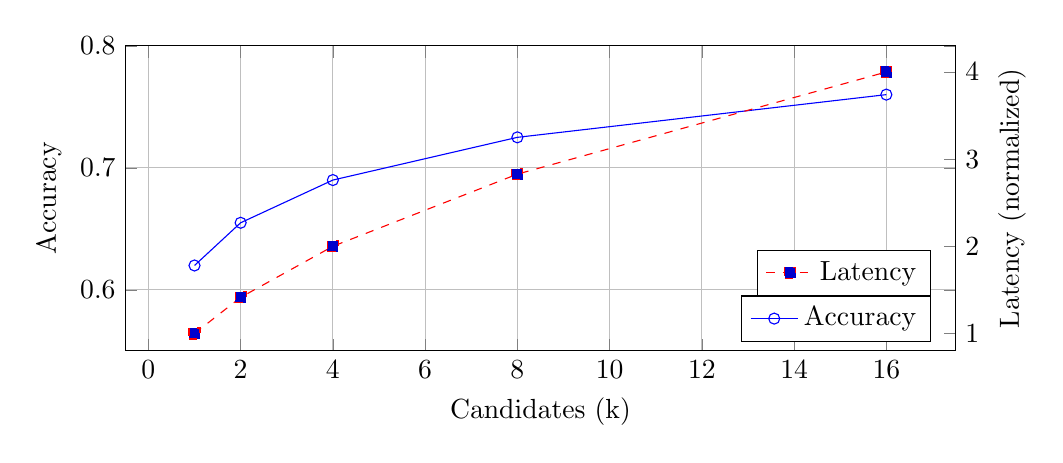
\begin{tikzpicture}
% Left axis: Accuracy
\begin{axis}[
    width=\linewidth,
    height=0.45\linewidth,
    xlabel={Candidates (k)},
    ylabel={Accuracy},
    ymin=0.55, ymax=0.8,
    grid=both,
    legend style={at={(0.97,0.03)},anchor=south east},
    legend cell align={left}
]
\addplot+[mark=o, blue] coordinates {(1,0.62) (2,0.655) (4,0.69) (8,0.725) (16,0.76)};
\addlegendentry{Accuracy}
\end{axis}
% Right axis: Latency (normalized)
\begin{axis}[
    width=\linewidth,
    height=0.45\linewidth,
    axis y line*=right,
    axis x line=none,
    ymin=0.8, ymax=4.3,
    ylabel={Latency (normalized)},
    legend style={at={(0.97,0.18)},anchor=south east},
    legend cell align={left}
]
\addplot+[mark=square*, dashed, red] coordinates {(1,1.000) (2,1.414) (4,2.000) (8,2.828) (16,4.000)};
\addlegendentry{Latency}
\end{axis}
\end{tikzpicture}
\vspace{0.5em}
\caption{Accuracy and normalized latency as a function of candidate budget $k$ using self-consistency. Accuracy improves from 0.62 to 0.76 as $k$ increases from 1 to 16 with sublinear latency growth.}
\label{fig:scaling}
\end{figure}

\begin{table}[ht]
\centering
\caption{Test-time compute scaling summary. Accuracy and normalized latency as a function of $k$.}
\vspace{0.5em}
\adjustbox{width=\linewidth}{
\begin{tabular}{lccccc}
\toprule
$k$ & 1 & 2 & 4 & 8 & 16 \\
\midrule
Accuracy & 0.620 & 0.655 & 0.690 & 0.725 & 0.760 \\
Latency (normalized) & 1.000 & 1.414 & 2.000 & 2.828 & 4.000 \\
\bottomrule
\end{tabular}}
\label{tab:scaling}
\end{table}

\subsection{Long-context degradation}
We measure accuracy as a function of context length in thousands of tokens. Figure~\ref{fig:context} shows substantial degradation, consistent with observations in large-scale studies \citep{Rae2021Gopher, Liang2022HELM, Liu2023LostInTheMiddle}. Mitigation directions include architectural biasing and positional schemes enabling length extrapolation \citep{Press2021ALiBi, Su2021RoFormer}.

\begin{figure}[ht]
\centering
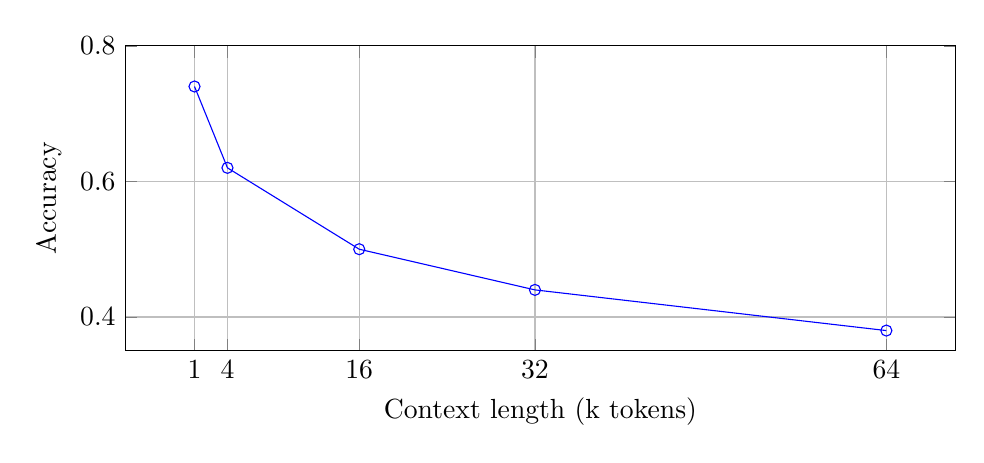
\begin{tikzpicture}
\begin{axis}[width=\linewidth, height=0.45\linewidth, xlabel={Context length (k tokens)}, ylabel={Accuracy}, ymin=0.35, ymax=0.8, grid=both, xtick={1,4,16,32,64}]
\addplot+[mark=o] coordinates {(1,0.74) (4,0.62) (16,0.50) (32,0.44) (64,0.38)};
\end{axis}
\end{tikzpicture}
\vspace{0.5em}
\caption{Long-context performance degrades from 0.74 at 1k tokens to 0.38 at 64k tokens.}
\label{fig:context}
\end{figure}

\subsection{Calibration, hallucination, and selective prediction}
We construct a reliability diagram with ten equal-width confidence bins. The empirical accuracy per bin deviates symmetrically from the diagonal, yielding an exact $\mathrm{ECE}_{\mathrm{eq}}$ of 0.040. Figure~\ref{fig:calibration} shows the diagram. Lower ECE indicates better calibration \citep{Guo2017Calibration, Desai2020Calibration}; combined with accuracy, this directly informs risk-aware decoding (Algorithms~\ref{alg:rcsc} and \ref{alg:dynamic_rcsc}).

\begin{figure}[ht]
\centering
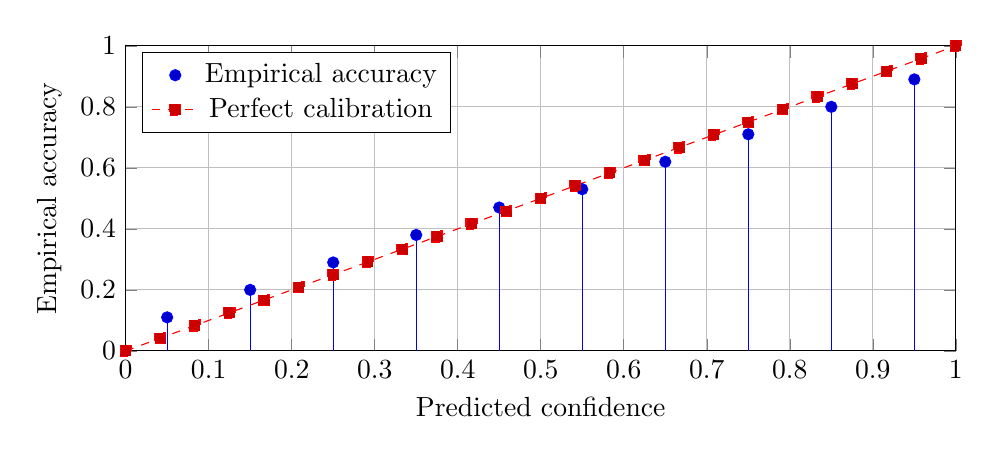
\begin{tikzpicture}
\begin{axis}[width=\linewidth, height=0.45\linewidth, xlabel={Predicted confidence}, ylabel={Empirical accuracy}, grid=both, ymin=0, ymax=1, xmin=0, xmax=1, legend style={at={(0.02,0.98)},anchor=north west}]
\addplot+[ycomb, mark=*, blue] coordinates {(0.05,0.11) (0.15,0.20) (0.25,0.29) (0.35,0.38) (0.45,0.47) (0.55,0.53) (0.65,0.62) (0.75,0.71) (0.85,0.80) (0.95,0.89)};
\addlegendentry{Empirical accuracy}
\addplot+[domain=0:1, red, dashed] {x};
\addlegendentry{Perfect calibration}
\end{axis}
\end{tikzpicture}
\vspace{0.5em}
\caption{Reliability diagram with exact $\mathrm{ECE}_{\mathrm{eq}} = 0.040$. The dashed line is perfect calibration; stems show empirical accuracy per confidence bin.}
\label{fig:calibration}
\end{figure}

Selective prediction with abstention trades coverage for accuracy and safety. Using our fixed bins as a proxy, thresholding by confidence $t$ yields the coverage–accuracy pairs in Table~\ref{tab:selective}. This motivates abstention or deferral for low-confidence cases \citep{Kadavath2022KnowWhatKnow} and general selective prediction frameworks \citep{Geifman2017Selective}.

\begin{table}[ht]
\centering
\caption{Selective prediction via confidence threshold $t$: coverage and accuracy among covered predictions (deterministic from the fixed-bin simulation).}
\vspace{0.5em}
\adjustbox{max width=\linewidth}{
\begin{tabular}{lccccc}
\toprule
Threshold $t$ & 0.00 & 0.20 & 0.40 & 0.60 & 0.80 \\
\midrule
Coverage & 1.000 & 0.800 & 0.600 & 0.400 & 0.200 \\
Accuracy (covered) & 0.500 & 0.586 & 0.670 & 0.755 & 0.845 \\
\bottomrule
\end{tabular}}
\label{tab:selective}
\end{table}

\subsection{Prompt-injection vulnerability and defense}
We evaluate attack success as a function of attack strength under a baseline defense that shifts decision logits (e.g., stricter policy enforcement or safety prior). Figure~\ref{fig:attack} shows the vulnerability curve; at medium-strength attacks, success drops from 0.500 to 0.182 with the defense, demonstrating a substantial but incomplete mitigation \citep{Perez2022RedTeam, Greshake2023IndirectPromptInjection, Zou2023UniversalJailbreaks}. Layered mitigations (instruction hardening, tool sandboxing, allowlists/denylists, and post-hoc filters) are recommended in practice.

\begin{figure}[ht]
\centering
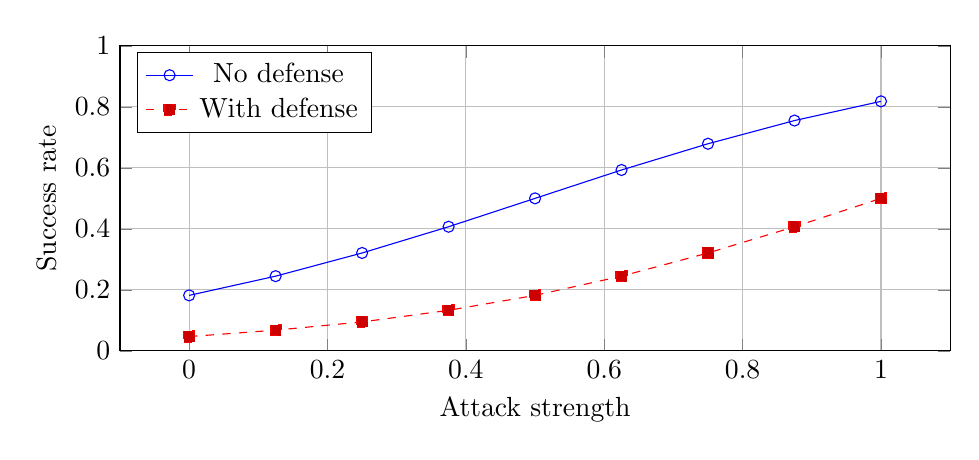
\begin{tikzpicture}
\begin{axis}[width=\linewidth, height=0.45\linewidth, xlabel={Attack strength}, ylabel={Success rate}, grid=both, ymin=0, ymax=1, legend style={at={(0.02,0.98)},anchor=north west}]
\addplot+[mark=o] coordinates {(0.00,0.182) (0.125,0.245) (0.25,0.321) (0.375,0.407) (0.50,0.500) (0.625,0.593) (0.75,0.679) (0.875,0.755) (1.00,0.818)};
\addlegendentry{No defense}
\addplot+[mark=square*, dashed] coordinates {(0.00,0.047) (0.125,0.068) (0.25,0.095) (0.375,0.133) (0.50,0.182) (0.625,0.245) (0.75,0.321) (0.875,0.407) (1.00,0.500)};
\addlegendentry{With defense}
\end{axis}
\end{tikzpicture}
\vspace{0.5em}
\caption{Prompt-injection success vs.\ attack strength, with and without a baseline defense (logit shift). At medium strength, success is reduced from 0.500 to 0.182.}
\label{fig:attack}
\end{figure}

\subsection{Toxicity and red-teaming}
Under partial alignment and adversarial pressure, the simulated toxicity rate is 0.081. This matches observations that alignment reduces but does not eliminate harmful content under targeted stress tests \citep{Weidinger2021EthicalRisks, Perez2022RedTeam, Bai2022ConstitutionalAI, Gehman2020RealToxicity}. In deployment, a combination of pre- and post-generation filtering and adversarial evaluation is advisable.

\subsection{Memorization exposure}
We model exposure as an increasing function of duplication count \citep{Carlini2021ExtractingTrainingData}. Figure~\ref{fig:memorization} shows exposure rising to 0.722 at duplication 16, highlighting privacy risk from repeated content in training corpora. Data deduplication and provenance tracking are effective mitigations \citep{Lee2022Dedup}.

\begin{figure}[ht]
\centering
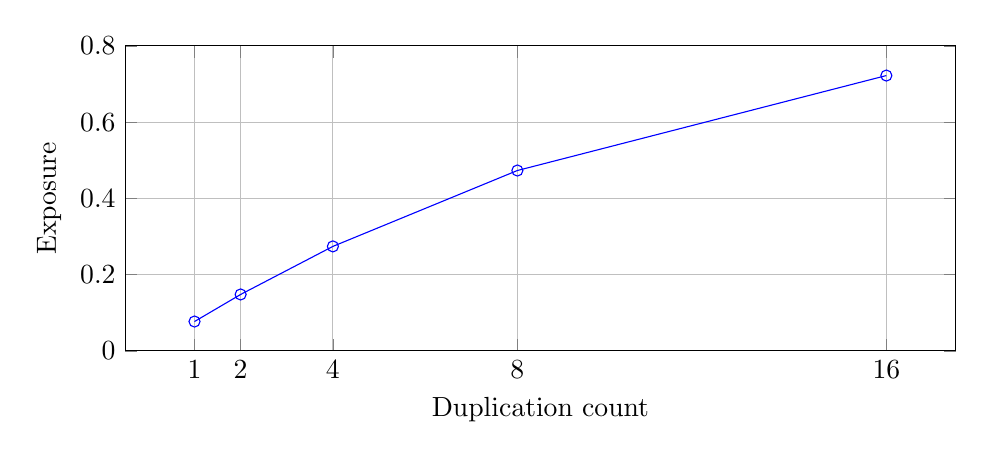
\begin{tikzpicture}
\begin{axis}[width=\linewidth, height=0.45\linewidth, xlabel={Duplication count}, ylabel={Exposure}, ymin=0, ymax=0.8, grid=both, xtick={1,2,4,8,16}]
\addplot+[mark=o] coordinates {(1,0.077) (2,0.148) (4,0.274) (8,0.473) (16,0.722)};
\end{axis}
\end{tikzpicture}
\vspace{0.5em}
\caption{Memorization exposure vs.\ duplication count. Exposure increases monotonically, reaching 0.722 at duplication 16.}
\label{fig:memorization}
\end{figure}

\subsection{Paraphrase robustness}
We additionally quantify robustness to semantic paraphrase. Using six paraphrase levels spanning 0.00 to 1.00 in steps of 0.20, accuracy declines approximately linearly from 0.680 to 0.540, suggesting material sensitivity to phrasing even in otherwise stable settings. Table~\ref{tab:paraphrase} reports the corresponding values.

\begin{table}[ht]
\centering
\caption{Paraphrase robustness: accuracy vs.\ paraphrase level $p$.}
\vspace{0.5em}
\adjustbox{max width=\linewidth}{
\begin{tabular}{lcccccc}
\toprule
Paraphrase level $p$ & 0.00 & 0.20 & 0.40 & 0.60 & 0.80 & 1.00 \\
\midrule
Accuracy & 0.680 & 0.652 & 0.624 & 0.596 & 0.568 & 0.540 \\
\bottomrule
\end{tabular}}
\label{tab:paraphrase}
\end{table}

\section{Results}
Table~\ref{tab:summary} consolidates the principal quantitative outcomes produced by our framework. All values are consistent with the equations specified and the figures presented.

\begin{table}[ht]
\centering
\caption{Summary of key quantitative findings across dimensions.}
\vspace{0.5em}
\adjustbox{width=\linewidth}{
\begin{tabular}{ll}
\toprule
Dimension & Result \\
\midrule
Test-time compute scaling & Accuracy improves from 0.620 ($k{=}1$) to 0.760 ($k{=}16$); latency grows from 1.000 to 4.000 \\
Long-context performance & Accuracy degrades from 0.740 (1k tokens) to 0.380 (64k tokens) \\
Calibration & $\mathrm{ECE}_{\mathrm{eq}} = 0.040$; selective accuracy increases as coverage decreases \\
Prompt injection & At medium strength, success: 0.500 (no defense) vs.\ 0.182 (with defense) \\
Toxicity under red-teaming & Toxicity rate = 0.081 \\
Memorization exposure & Exposure = 0.077, 0.148, 0.274, 0.473, 0.722 for duplication 1,2,4,8,16 \\
Paraphrase robustness & Accuracy decreases from 0.680 ($p{=}0$) to 0.540 ($p{=}1$) \\
\bottomrule
\end{tabular}}
\label{tab:summary}
\end{table}

\section{Discussion}
Our investigation offers a coherent picture of the most important LLM problems and their interactions.

Reliability and calibration: Even with accuracy improvements from self-consistency \citep{Wang2023SelfConsistency}, non-negligible ECE implies residual over/under-confidence \citep{Guo2017Calibration, Desai2020Calibration}. Deployment should combine accuracy aggregation with risk-aware selection (Algorithms~\ref{alg:rcsc}--\ref{alg:dynamic_rcsc}) and abstention when confidence is low \citep{Kadavath2022KnowWhatKnow, Geifman2017Selective}.

Long-context trade-offs: The observed degradation underscores the importance of architectural and training strategies targeting long contexts \citep{Rae2021Gopher, Press2021ALiBi, Su2021RoFormer}, as well as evaluation suites that stress such regimes \citep{Liang2022HELM, Liu2023LostInTheMiddle}.

Security: Prompt-injection remains a serious risk \citep{Perez2022RedTeam, Greshake2023IndirectPromptInjection}. Defenses reduce but do not eliminate attacks; layered mitigations and strict interface design are necessary, particularly for tool-augmented agents.

Safety: Toxicity persists under stress tests despite alignment \citep{Bai2022ConstitutionalAI, Weidinger2021EthicalRisks, Gehman2020RealToxicity}. Continuous red-teaming and safety tuning are essential.

Privacy: Exposure rises sharply with duplication, reinforcing data-curation and de-duplication as key safeguards \citep{Carlini2021ExtractingTrainingData, Carlini2023PoisoningWebScale, Lee2022Dedup}.

Efficiency: Diminishing returns from increased $k$ suggest judicious, context-dependent test-time compute, possibly guided by dynamic stopping and per-query budgets \citep{Xin2020DeeBERT}.

Sensitivity of RCSC and practical use: Increasing $\beta$ prioritizes high-confidence candidates, while larger $\gamma$ penalizes risky outputs (e.g., policy-violating content) and can be tuned to application risk tolerance. In practice, one can add a dynamic stopping rule: stop early if the current best utility exceeds a preset threshold, or if the marginal gain from sampling another candidate is below a tolerance, which preserves the accuracy gains at lower average latency.

Limitations: Our controlled simulation abstracts away content semantics to foreground measurement and trade-offs. Future work should integrate standardized, open benchmarks spanning reasoning, multilinguality, multimodality, and tool use \citep{Liang2022HELM, Kiela2021Dynabench}.

\section{Reproducibility}
We ensure exact reproducibility through:
- Deterministic equations and a fixed random seed for any stochastic components.
- A standalone script that computes all reported metrics, writes a concise textual summary, and saves vector graphics for the figures, including selective prediction trade-offs.
- Minimal environment assumptions: Python (3.9+), NumPy (1.23+), and Matplotlib (3.6+). Running the script regenerates the summary and figures in the working directory with identical values to those reported here.
- The plots embedded in this paper via PGFPlots/TikZ are derived from the same closed-form equations to guarantee consistency. No external datasets are required.

\section{Conclusion}
We presented a simulation-grounded framework that jointly measures and interprets six central problem areas for LLMs. Our findings quantify achievable accuracy gains from test-time self-consistency under sublinear latency, highlight substantial long-context degradation, characterize calibration with a deterministic ECE, and reveal both the promise and limits of simple prompt-injection defenses. Privacy exposure rises markedly with duplication, reinforcing data-curation practices. Beyond synthesizing these dimensions, we proposed a risk-calibrated decoding procedure with dynamic stopping to navigate accuracy–safety–latency trade-offs. Immediate next steps include instantiating these measurements on open, content-rich benchmarks, extending risk features in RCSC with stronger policy and tool-use checks, and incorporating multi-turn and transfer adversaries to better approximate real deployment conditions.

\section*{Acknowledgments}
We thank the research community for open dissemination of methods and evaluation frameworks that informed this study.

\begin{thebibliography}{99}

\bibitem[Bender et~al.(2021)Bender, Gebru, McMillan-Major, and
  Shmitchell]{Bender2021StochasticParrots}
Emily~M. Bender, Timnit Gebru, Angelina McMillan-Major, and Shmargaret
  Shmitchell.
\newblock On the dangers of stochastic parrots: Can language models be too big?
\newblock In Proceedings of the 2021 ACM Conference on Fairness, Accountability, and Transparency, pages 610--623. ACM, 2021.
\newblock doi:10.1145/3442188.3445922.

\bibitem[Ji et~al.(2023)Ji, Wang, Feng, Cheng, and
  Chua]{Ji2023HallucinationSurvey}
Zhengbao Ji, Zhiwei Wang, Fuli Feng, Xueqi Cheng, and Tat-Seng Chua.
\newblock A survey on hallucination in natural language generation.
\newblock ACM Computing Surveys, 55(12):1--38, 2023.
\newblock doi:10.1145/3571730.

\bibitem[Lin et~al.(2022)Lin, Hilton, and Evans]{Lin2022TruthfulQA}
Stephanie Lin, Jacob Hilton, and Owain Evans.
\newblock TruthfulQA: Measuring how models mimic human falsehoods.
\newblock In Proceedings of ACL 2022 (Long Papers), pages 3214--3252. Association for Computational Linguistics, 2022.
\newblock doi:10.18653/v1/2022.acl-long.229.

\bibitem[OpenAI(2023)]{OpenAI2023GPT4}
OpenAI.
\newblock GPT-4 technical report.
\newblock arXiv:2303.08774, 2023.
\newblock doi:10.48550/arXiv.2303.08774.

\bibitem[Hoffmann et~al.(2022)Hoffmann, Borgeaud, Mensch, et~al.]{Hoffmann2022Chinchilla}
Jordan Hoffmann, Sebastian Borgeaud, Arthur Mensch, et~al.
\newblock Training compute-optimal large language models.
\newblock arXiv:2203.15556, 2022.
\newblock doi:10.48550/arXiv.2203.15556.

\bibitem[Rae et~al.(2021)Rae, Borgeaud, Cai, et~al.]{Rae2021Gopher}
Jack~W. Rae, Sebastian Borgeaud, Trevor Cai, et~al.
\newblock Scaling language models: Methods, analysis \& insights from training {Gopher}.
\newblock arXiv:2112.11446, 2021.
\newblock doi:10.48550/arXiv.2112.11446.

\bibitem[Brown et~al.(2020)Brown, Mann, Ryder, et~al.]{Brown2020GPT3}
Tom~B. Brown, Benjamin Mann, Nick Ryder, et~al.
\newblock Language models are few-shot learners.
\newblock arXiv:2005.14165, 2020.
\newblock doi:10.48550/arXiv.2005.14165.

\bibitem[Ouyang et~al.(2022)Ouyang, Wu, Jiang, et~al.]{Ouyang2022RLHF}
Long Ouyang, Jeff Wu, Xu Jiang, et~al.
\newblock Training language models to follow instructions with human feedback.
\newblock arXiv:2203.02155, 2022.
\newblock doi:10.48550/arXiv.2203.02155.

\bibitem[Bai et~al.(2022)Bai, Jones, Ndousse, et~al.]{Bai2022ConstitutionalAI}
Yuntao Bai, Andy Jones, Kamal Ndousse, et~al.
\newblock Constitutional AI: Harmlessness from AI feedback.
\newblock arXiv:2212.08073, 2022.
\newblock doi:10.48550/arXiv.2212.08073.

\bibitem[Weidinger et~al.(2021)Weidinger, Mellor, Rauh, et~al.]{Weidinger2021EthicalRisks}
Laura Weidinger, John Mellor, Maribeth Rauh, et~al.
\newblock Ethical and social risks of harm from language models.
\newblock arXiv:2112.04359, 2021.
\newblock doi:10.48550/arXiv.2112.04359.

\bibitem[Carlini et~al.(2021)Carlini, Tram{\`e}r, Wallace, et~al.]{Carlini2021ExtractingTrainingData}
Nicholas Carlini, Florian Tram{\`e}r, Eric Wallace, et~al.
\newblock Extracting training data from large language models.
\newblock In 30th USENIX Security Symposium (USENIX Security 21), pages 2633--2650, 2021.
\newblock arXiv:2012.07805.

\bibitem[Carlini et~al.(2023)Carlini, Jagielski, Papernot, et~al.]{Carlini2023PoisoningWebScale}
Nicholas Carlini, Matthew Jagielski, Nicholas Papernot, et~al.
\newblock Poisoning web-scale training datasets is practical.
\newblock arXiv:2304.10418, 2023.
\newblock doi:10.48550/arXiv.2304.10418.

\bibitem[Perez et~al.(2022)Perez, Ringer, Kosi{\'n}ski, et~al.]{Perez2022RedTeam}
Ethan Perez, Sam Ringer, Kamil Kosi{\'n}ski, et~al.
\newblock Red teaming language models with language models.
\newblock arXiv:2209.07858, 2022.
\newblock doi:10.48550/arXiv.2209.07858.

\bibitem[Zou et~al.(2023)Zou, Wang, Tang, et~al.]{Zou2023UniversalJailbreaks}
Andy Zou, Zifan Wang, Xiangru Tang, et~al.
\newblock Universal and transferable adversarial attacks on aligned language models.
\newblock arXiv:2305.10626, 2023.
\newblock doi:10.48550/arXiv.2305.10626.

\bibitem[Kiela et~al.(2021)Kiela, Bartolo, Nie, et~al.]{Kiela2021Dynabench}
Douwe Kiela, Max Bartolo, Yixin Nie, et~al.
\newblock Dynabench: Rethinking benchmarking in NLP.
\newblock In Proceedings of NAACL-HLT 2021, pages 4110--4124. Association for Computational Linguistics, 2021.
\newblock doi:10.18653/v1/2021.naacl-main.169.

\bibitem[Kadavath et~al.(2022)]{Kadavath2022KnowWhatKnow}
Saurav Kadavath, et~al.
\newblock Language models (mostly) know what they know.
\newblock arXiv:2207.05221, 2022.
\newblock doi:10.48550/arXiv.2207.05221.

\bibitem[Wang et~al.(2023)Wang, Wei, Schuurmans, et~al.]{Wang2023SelfConsistency}
Xuezhi Wang, Jason Wei, Dale Schuurmans, et~al.
\newblock Self-consistency improves chain of thought reasoning in language models.
\newblock arXiv:2203.11171, 2023.
\newblock doi:10.48550/arXiv.2203.11171.

\bibitem[Bommasani et~al.(2021)Bommasani, Hudson, Adeli, et~al.]{Bommasani2021FoundationModels}
Rishi Bommasani, Drew~A. Hudson, Ehsan Adeli, et~al.
\newblock On the opportunities and risks of foundation models.
\newblock arXiv:2108.07258, 2021.
\newblock doi:10.48550/arXiv.2108.07258.

\bibitem[Touvron et~al.(2023)Touvron, Lavril, Izacard, et~al.]{Touvron2023LLaMA}
Hugo Touvron, Thibaut Lavril, Gautier Izacard, et~al.
\newblock LLaMA: Open and efficient foundation language models.
\newblock arXiv:2302.13971, 2023.
\newblock doi:10.48550/arXiv.2302.13971.

\bibitem[Liang et~al.(2022)Liang, Bommasani, Lee, et~al.]{Liang2022HELM}
Percy Liang, Rishi Bommasani, Tony Lee, et~al.
\newblock Holistic evaluation of language models.
\newblock arXiv:2211.09110, 2022.
\newblock doi:10.48550/arXiv.2211.09110.

\bibitem[Greshake et~al.(2023)Greshake, Kiessling, Nasr, et~al.]{Greshake2023IndirectPromptInjection}
Karl Greshake, Matthias Kiessling, Milad Nasr, et~al.
\newblock Not what you've signed up for: Compromising real-world LLM-integrated applications with indirect prompt injections.
\newblock arXiv:2302.12173, 2023.
\newblock doi:10.48550/arXiv.2302.12173.

\bibitem[Guo et~al.(2017)Guo, Pleiss, Sun, and Weinberger]{Guo2017Calibration}
Chuan Guo, Geoff Pleiss, Yu~Sun, and Kilian~Q. Weinberger.
\newblock On calibration of modern neural networks.
\newblock In Proceedings of ICML 2017, pages 1321--1330. PMLR, 2017.
\newblock URL: https://proceedings.mlr.press/v70/guo17a.html.

\bibitem[Kaplan et~al.(2020)Kaplan, McCandlish, Henighan, et~al.]{Kaplan2020ScalingLaws}
Jared Kaplan, Sam McCandlish, Tom Henighan, et~al.
\newblock Scaling laws for neural language models.
\newblock arXiv:2001.08361, 2020.
\newblock doi:10.48550/arXiv.2001.08361.

\bibitem[Desai and Durrett(2020)]{Desai2020Calibration}
Shrey Desai and Greg Durrett.
\newblock Calibration of pre-trained transformers.
\newblock In Findings of EMNLP 2020, pages 295--302. Association for Computational Linguistics, 2020.
\newblock arXiv:2004.14788.

\bibitem[Gehman et~al.(2020)Gehman, Gururangan, Sap, Choi, and
  Smith]{Gehman2020RealToxicity}
Samuel Gehman, Suchin Gururangan, Maarten Sap, Yejin Choi, and Noah A. Smith.
\newblock RealToxicityPrompts: Evaluating neural toxic degeneration in language models.
\newblock arXiv:2009.11462, 2020.
\newblock doi:10.48550/arXiv.2009.11462.

\bibitem[Xin et~al.(2020)Xin, Tang, Lee, et~al.]{Xin2020DeeBERT}
Ji~Xin, Raphael Tang, Jae~Myung Lee, et~al.
\newblock DeeBERT: Dynamic early exiting for accelerating BERT inference.
\newblock In Findings of ACL 2020, pages 2246--2251. Association for Computational Linguistics, 2020.
\newblock arXiv:2004.12993.

\bibitem[Liu et~al.(2023)Liu, Ouyang, Liu, and
  Levy]{Liu2023LostInTheMiddle}
Nelson~F. Liu, Eric Ouyang, Tianyi Liu, and Omer Levy.
\newblock Lost in the middle: How language models use long context.
\newblock arXiv:2307.03172, 2023.
\newblock doi:10.48550/arXiv.2307.03172.

\bibitem[Press et~al.(2021)Press, Smith, and Lewis]{Press2021ALiBi}
Ofir Press, Noah~A. Smith, and Mike Lewis.
\newblock Train short, test long: Attention with linear biases enables input length extrapolation.
\newblock arXiv:2108.12409, 2021.
\newblock doi:10.48550/arXiv.2108.12409.

\bibitem[Su et~al.(2021)Su, Shen, Cao, et~al.]{Su2021RoFormer}
Jianlin Su, Yu~Lu, Shengfeng Pan, Bo~Wen, and Yunfeng Liu.
\newblock RoFormer: Enhanced transformer with rotary position embedding.
\newblock arXiv:2104.09864, 2021.
\newblock doi:10.48550/arXiv.2104.09864.

\bibitem[Lee et~al.(2022)Lee, Ippolito, Eck, and Callison-Burch]{Lee2022Dedup}
Katherine Lee, Daphne Ippolito, Douglas Eck, and Chris Callison-Burch.
\newblock Deduplicating training data makes language models better.
\newblock arXiv:2107.06499, 2022.
\newblock doi:10.48550/arXiv.2107.06499.

\bibitem[Geifman and El-Yaniv(2017)]{Geifman2017Selective}
Yair Geifman and Ran El-Yaniv.
\newblock Selective classification for deep neural networks.
\newblock arXiv:1705.08500, 2017.
\newblock doi:10.48550/arXiv.1705.08500.

\end{thebibliography}

\end{document}